\documentclass{article}
\usepackage[utf8]{inputenc}
\usepackage[T1]{fontenc}
\usepackage{array}
\usepackage{url}
\usepackage{graphicx}
\usepackage{amsmath}
\usepackage{alltt}
\usepackage{multicol}

\author{Philip Pickering\\\url{pgpick@gmx.at} \and Thomas Bracht Laumann Jespersen\\\url{ntl316@alumni.ku.dk}}
\title{Advanced Algorithms and Data Structures\\Hand-in 1}
\date{}


\setcounter{MaxMatrixCols}{20}
\begin{document}
\maketitle

The problem could be formulated and solved as a max-flow
problem. There are a few things to observe before that: the network
(as in the example) is undirected, in which case we would want to make
it directed. We also have several sources that may themselves be
connected (such as nodes 2 and 3 in the example).

%%  Let the network be an undirected graph called $N = (V,E)$. We want to
%% construct a max-flow graph $G = (V_G, E_G)$ from $N$. For all the
%% edges $u,v \in V$, we let $u,v \in V_G$, and $(u,v), (v,u) \in
%% E_G$. If we let $k$ denote the capacity of the edge $(u,v)\in E$, then
%% we let $c(u,v) = c(v,u) = k$ in $G$. Finally we attach a common source
%% to all the nodes that were sources in $N$, call it $s$, and we let
%% $c(s,u) = \infty$ for all the nodes $u$ that were sources in $N$.

Let the network be an undirected graph called $N = (V,E)$. We want to
construct a max-flow graph $G = (V',E')$ from $N$. For all nodes
$u,v\in V$ and $(u,v)\in E$, we add to our max-flow 
graph nodes $u, v$ and an extra node $w$. We add add directed edges
$(u,v), (v,w)$ and $(w,u)$. If we let $k$ denote the capacity of the
edge $(u,v)\in E$, then we let $c(u,v) = c(v,w) = c(w,u) = k$ in
$G$. Lastly, we add a super source $s$ and an edge $(s,v)$ to all the
nodes $v$ that were a source in $N$.

The number of edges in $G$ is $|V'| = |V| + |E| + 1 $ and $|E'| = 3|E|
+ p$, where $p$ is the number of edges added from the super source
$s$. $p$ is exactly the number of sources in $N$.

Now we have the original problem stated as a max-flow problem, which
can be easily expressed as a linear program

\[
\begin{array}{lrcll}
\textrm{max.:} & \displaystyle\sum_{v\in V_G} f(s,v) -\displaystyle\sum_{v\in V_G} f(v,s) &     & & \\
\textrm{s.t.:} &  f(u,v)                &\leq & c(u,v),  &\forall u,v\in V_G\\
              &  \displaystyle\sum_{v\in V_G}f(v,u) -\displaystyle\sum_{v\in V_G}f(u,v)                & =   & 0 &\forall u,v\in V_G\\
              & f(u,v) & = & 0, &\forall u,v\in V_G
\end{array}
\]

As small example graph can be found in fig.\ref{fig:exg}.

\begin{figure}
  \centering
  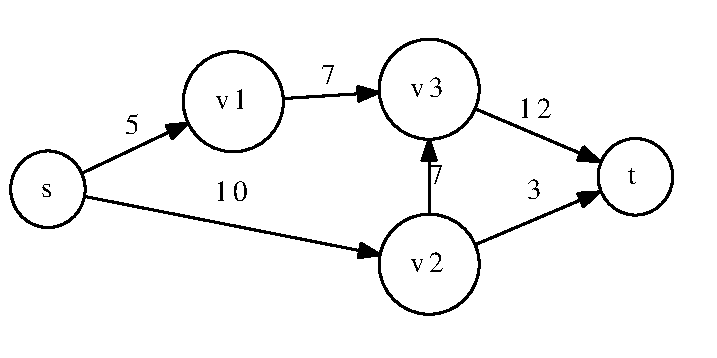
\includegraphics[width=.7\textwidth]{exg.pdf}
  \caption{An example max-flow graph}
  \label{fig:exg}
\end{figure}

The linear program corresponding to the graph in fig.~\ref{fig:exg} is
the following:
\[
\begin{array}{lrcll}
\textrm{max.:} & f_{s,v_1} + f_{s,v_2} & & &\\
\textrm{s.t.:} & f_{s,v_1} &\leq & c(s,v_1) = 5&\\
               & f_{s,v_2} &\leq & c(s,v_2) = 10&\\
               & f_{v_1,v_3} &\leq & c(v_1,v_3) = 7&\\
               & f_{v_2,v_3} &\leq & c(v_1,v_3) = 7&\\
               & f_{v_2,t} &\leq & c(v_2,t) = 3&\\
               & f_{v_3,t} &\leq & c(v_3,t) = 12&\\
               & f_{s,v_1} &= &f_{v_1,v_3}&\\
               & f_{s,v_2} &= &f_{v_2,v_3} + f_{v_2,t}&\\
               & f_{v_1,v_3} + f_{v_2,v_3} &= &f_{v_3,t}&\\
& f_{s,v_1}, f_{s,v_2},f_{v_1,v_3},f_{v_2,v_3},f_{v_2,t}, f_{v_3,t} & \geq & 0\\
\end{array}
\]

We have minimized the above linear program, such that edges with
capacity zero have been omitted. Without showing the work of the
simplex algorithm, we arrive at the solution: $f_{s,v_1} = 5, f_{s,v_2} =
10$.

\section*{\hfill}

In order to find the cheapest critical connection we have to identify
the \emph{minimal cuts}. Intuitively, if we have a cut $(S, T)$ of our
graph and a maximum flow $f$ in that same graph, then the flow from
$S$ to $T$ must be equal to capacity across that cut, $c(S,T)$. This
means in order to increase the overall flow of the graph, we have to
increase the capacities on some of the edges of our minimal cuts.

If we only have one such minimal cut, then we simply select the edge
with the smallest capacity and increase its capacity. If we have more
than one cut, it's not immediately clear which edges to choose.
In our example above, we can identify three minimal cuts:
\begin{enumerate}
  \item $S_1 = \{s\}$, $T_1 = V - \{s\}$
  \item $S_2 = \{s,v_2\}$, $T_2 = \{v_1,v_3,t \}$
  \item $S_3 = V - \{t\}$, $T_3 = \{t\}$.
\end{enumerate}

In the first cut we can identify the edge $(s, v_1)$, $c(s,v_1) = 5$,
as the cheapest to increase, for $(S_2,T_2)$ the cheapest edge is
$(v_2,t)$, $c(v_2,t) = 3$, and this is also the cheapest to increase
for $(S_3, T_3)$. If we increase the capacities of these two edges by
1, then we have increased the capacities of all the minimal cuts
$(S_i,T_i)$ by 1. In this example the above cuts are still minimal
cuts, so the max-flow min-cut theorem tells us that we have increased
the maximum flow by 1 (otherwise we should have provoked another
minimal cut).

Recaptured briefly, in order to find the ``cheapest critical
connection'', we need to inspect the minimal cuts and for each of
them, select the edge with the smallest capacity to increase. In the
end, by the max-flow min-cut property, we will have increased the
maximum flow in the entire graph.

\section*{\hfill}

The dual of the above stated problem can be stated by restating the
above program in standard form $Ax\leq b$ along with a coefficent
vector $c = \begin{pmatrix} 1 & 1 & 0 & 0 & 0 & 0\end{pmatrix}^T$. The
  dual is then given by $A^Ty \geq c$, where we minimize $b^Ty$. $y$
  is a vector of size proportional to the number of constraints, in
  our case 12, because each of the equality constraints give rise to
  two inequalities. Now we can state the dual:

\[
\begin{array}{cl}
\textrm{min.:} & 5y_1 + 10y_2 + 7y_3 + 7y_4 + 3y_5 + 12y_6\\
\textrm{s.t.:} &
 \begin{bmatrix}%
 1 & 0 & 0 & 0 & 0 & 0 & 1 & -1 & 0 & 0 & 0 & 0\\
 0 & 1 & 0 & 0 & 0 & 0 & 0 & 0 & 1 & -1 & 0 & 0\\
 0 & 0 & 1 & 0 & 0 & 0 & -1 & 1 & 0 & 0 & 1 & -1\\
 0 & 0 & 0 & 1 & 0 & 0 & 0 & 0 & -1 & 1 & 1 & -1\\
 0 & 0 & 0 & 0 & 1 & 0 & 0 & 0 & -1 & 1 & 0 & 0\\
 0 & 0 & 0 & 0 & 0 & 1 & 0 & 0 & 0 & 0 & -1 & 1
\end{bmatrix}y
\geq
\begin{pmatrix}
  1\\ 1\\ 0\\ 0\\ 0\\ 0
\end{pmatrix}
%%\begin{pmatrix} 1\\ 2\end{pmatrix}
\end{array}
\]
A solution to the dual problem is $y_1 = 1, y_2 = 1$ and the rest are
zero.

\section*{\hfill}
%% \begin{quotation}\itshape
%% Some of the relay stations are not owned by the company, so they have
%% to pay a leasing price of 1 øre for each byte transferred in and out
%% of the company’s network (see Figure 2 for an example).  

%% Assuming that the company has already determined the maximum transfer
%% rate, and wants to maintain this, give a linear program that finds the
%% lowest possible price they will have to pay for it.
%% \end{quotation}

In order to model that some of the relay stations aren't owned by
the company, we can rephrase the problem as a \emph{minimum-cost flow}
problem (Cormen 29.51, pg 862), where the cost function is defined by:

\[
a(u,v) = \left\{\begin{array}{ll}1,&\text{if $u$ xor $v$ is not owned
  by the company}\\ 0,&\text{otherwise.}\end{array}\right.
\]
Then we can directly apply the definition from the book, because we
can require the value of the flow to be exactly $d$.


\section*{Results}
\subsection*{Obtaining results}
Using the provided \emph{Network.java}, the following steps were taken to obtain the results:
\begin{enumerate}
\item The given network was converted to a maximum flow graph
\item Then it was further transformed into a linear program: As described in Corman, pg 860, an objective function and constraints for the capacities and the flow conservation have been generated.
\item The objective function was set to be maximized.
\item This LP has been solved using \emph{lp\_solve} with the Java wrapper. 
\end{enumerate}
The returned result was the maximum flow and represented the largest bit rate. For solving the problem of the lowest leasing rate, the linear program has been modified to a minimum cost flow problem (see Cormen pg 861):
\begin{enumerate}
\item The previous objective function was used as the LHS of a new constraint, the previous result was used as the RHS.
\item A cost matrix was created and transformed into a form to match the converted network.
\item A new objective function using the cost matrix was generated.
\item The new LP minimized the objective function.
\end{enumerate}
This returned the minimum costs for leasing while maintaining the transfer rate. 

See attached Java files, especially \emph{MF.java} and the modified \emph{Network.java}, also see a simpler network which represents the example from above in \emph{SmallNet.java}. 

The following is the relevant part of the output of the calculations on the given network.
\subsection*{Largest bit rate}
\begin{multicols}{2}
\begin{alltt}
Max Flow: 95.0
Flow[([S])(0[s])] = 30.0
Flow[([S])(1[s])] = 10.0
Flow[([S])(2[s])] = 25.0
Flow[([S])(3[s])] = 5.0
Flow[([S])(4[s])] = 15.0
Flow[([S])(5[s])] = 10.0
Flow[(0[s])(6)] = 20.0
Flow[(0[s])(7)] = 10.0
Flow[(1[s])(8)] = 10.0
Flow[(2[s])(9)] = 25.0
Flow[(3[s])(9)] = 5.0
Flow[(4[s])(9)] = 5.0
Flow[(4[s])(10)] = 10.0
Flow[(5[s])(10)] = 10.0
Flow[(6)(18)] = 20.0
Flow[(7)(18)] = 10.0
Flow[(8)(12)] = 10.0
Flow[(9)(11)] = 15.0
Flow[(9)(12)] = 20.0
Flow[(10)(11)] = 20.0
Flow[(11)(13)] = 15.0
Flow[(11)(14)] = 20.0
Flow[(12)(15)] = 30.0
Flow[(13)(14)] = 10.0
Flow[(13)(15)] = 5.0
Flow[(14)(19[t])] = 30.0
Flow[(15)(16)] = 10.0
Flow[(15)(19[t])] = 30.0
Flow[(16)(19[t])] = 35.0
Flow[(17)(23)] = 10.0
Flow[(18)(20)] = 10.0
Flow[(18)(21)] = 10.0
Flow[(18)(18/17)] = 10.0
Flow[(20)(22)] = 10.0
Flow[(21)(22)] = 20.0
Flow[(22)(24)] = 30.0
Flow[(23)(23/21)] = 10.0
Flow[(24)(24/15)] = 5.0
Flow[(24)(24/16)] = 25.0
Flow[(24/15)(15)] = 5.0
Flow[(24/16)(16)] = 25.0
Flow[(18/17)(17)] = 10.0
Flow[(23/21)(21)] = 10.0

\end{alltt}
\end{multicols}

\subsection*{Lowest leasing price}
\begin{multicols}{2}
\begin{alltt}
Minimum Cost: 60.0
Flow[([S])(0[s])] = 30.0
Flow[([S])(1[s])] = 10.0
Flow[([S])(2[s])] = 25.0
Flow[([S])(3[s])] = 5.0
Flow[([S])(4[s])] = 15.0
Flow[([S])(5[s])] = 10.0
Flow[(0[s])(6)] = 20.0
Flow[(0[s])(7)] = 10.0
Flow[(1[s])(8)] = 10.0
Flow[(2[s])(9)] = 25.0
Flow[(3[s])(9)] = 5.0
Flow[(4[s])(9)] = 5.0
Flow[(4[s])(10)] = 10.0
Flow[(5[s])(10)] = 10.0
Flow[(6)(18)] = 20.0
Flow[(7)(18)] = 10.0
Flow[(8)(12)] = 10.0
Flow[(9)(11)] = 15.0
Flow[(9)(12)] = 20.0
Flow[(10)(11)] = 20.0
Flow[(11)(13)] = 15.0
Flow[(11)(14)] = 20.0
Flow[(12)(15)] = 30.0
Flow[(13)(14)] = 5.0
Flow[(13)(15)] = 10.0
Flow[(14)(19[t])] = 25.0
Flow[(15)(16)] = 10.0
Flow[(15)(19[t])] = 30.0
Flow[(16)(19[t])] = 40.0
Flow[(17)(23)] = 10.0
Flow[(18)(20)] = 10.0
Flow[(18)(21)] = 10.0
Flow[(18)(18/17)] = 10.0
Flow[(20)(22)] = 10.0
Flow[(21)(22)] = 10.0
Flow[(22)(24)] = 20.0
Flow[(23)(24)] = 10.0
Flow[(24)(24/16)] = 30.0
Flow[(24/16)(16)] = 30.0
Flow[(18/17)(17)] = 10.0

\end{alltt}
\end{multicols}

%% \newpage
%% \begin{enumerate}
%% \item Give a precise explanation how the company could efficiently determine
%% the largest transfer rate to the server. 

%% \item Write a linear program that finds this transfer rate

%% \item Give a small example graph and write the optimal solution to the
%% linear program given above.  

%% \item The cost of increasing the capacity of a connection with one unit is
%% directly proportional to the capacity of that connection.  

%% Give a precise explanation how the company could efficiently determine
%% the cheapest 'critical connection' to improve in order to get a better
%% maximum transfer rate from the workstations to the server.  

%% \item Write the dual of the linear program you gave before and find the
%% optimal solution in the example you created before.   

%% \item How could the critical connections be determined from the dual?

%% \item Some of the relay stations are not owned by the company, so they have
%% to pay a leasing price of 1 øre for each byte transferred in and out
%% of the company’s network (see Figure 2 for an example).  

%% Assuming that the company has already determined the maximum transfer
%% rate, and wants to maintain this, give a linear program that finds the
%% lowest possible price they will have to pay for it.

%% \item Attached is a Java class (Network.java) specifying a network as just
%% described.

%% Report both the largest bit rate and the lowest leasing-price for this
%% problem and give a brief description of how you obtained this
%% result. It is preferrable if you use a linear programming package that
%% can be called from your programming language of choice. The second
%% assignment will require this as well. 
%% \end{enumerate}

\end{document}
